\documentclass[letterpaper,11pt]{article}

% --- Packages ---
\usepackage[margin=1in]{geometry}
\usepackage{amsmath,amssymb,amsthm}
\usepackage{mathtools}
\usepackage{microtype}
\usepackage{booktabs}
\usepackage{multirow}
\usepackage{enumitem}
\usepackage{hyperref}
\usepackage{cleveref}
\usepackage{algorithm}
\usepackage{algorithmic}
\usepackage{pgfplots}
\usepackage{tikz}
\usetikzlibrary{arrows.meta,positioning,calc,patterns,decorations.markings}
\pgfplotsset{compat=1.18}

% --- Theorem environments ---
\newtheorem{theorem}{Theorem}
\newtheorem{proposition}[theorem]{Proposition}
\newtheorem{lemma}[theorem]{Lemma}
\newtheorem{corollary}[theorem]{Corollary}
\newtheorem{definition}[theorem]{Definition}
\newtheorem{remark}[theorem]{Remark}

% --- Commands ---
\DeclareMathOperator{\Aut}{Aut}
\DeclareMathOperator{\Cl}{Cl}
\DeclareMathOperator{\diag}{diag}
\DeclareMathOperator{\MSE}{MSE}
\DeclareMathOperator{\NSM}{NSM}
\newcommand{\R}{\mathbb{R}}
\newcommand{\C}{\mathbb{C}}
\newcommand{\HH}{\mathbb{H}}
\newcommand{\OO}{\mathbb{O}}
\newcommand{\norm}[1]{\lVert #1 \rVert}
\newcommand{\inner}[2]{\langle #1, #2 \rangle}
\newcommand{\conj}[1]{\overline{#1}}

\title{Structured Rotations and Lattice Quantization\\for KV Cache Compression\\via Cayley-Dickson Algebra}
\author{Oichkatzelesfrettschen}
\date{March 2026}

\begin{document}
\maketitle

\begin{abstract}
We extend TurboQuant (ICLR 2026), a two-stage KV cache quantizer for
large language models, with structured rotations derived from
Cayley-Dickson (CD) algebra and E8 lattice quantization.
Our full-stack pipeline---NSN pre-processing, Walsh-Hadamard rotation
via cuBLAS, Lloyd-Max quantization, and bit-packed QJL correction---achieves
$+$136 basis points cosine similarity improvement and 69\% memory reduction
over vanilla TurboQuant on Qwen2.5-3B and Mistral-7B.
We establish a unified algebraic framework connecting CD algebras,
Clifford algebras $\Cl(p,q)$, the E8 root lattice, and the
Barnes-Wall hierarchy, with 30 of 36 provable properties
formally verified via Z3 SMT solver. Ablation reveals that NSN
pre-processing---not the rotation method---is the dominant contributor,
while CD algebraic structure provides formal isometry guarantees that
constrain quantization error geometry.
Code: \texttt{github.com/Oichkatzelesfrettschen/turboquant-pytorch}
\end{abstract}

% =====================================================================
\section{Introduction}
% =====================================================================

Key-value (KV) cache memory is the primary bottleneck for long-context
LLM inference. TurboQuant~\cite{turboquant2026} addresses this via
random orthogonal rotation followed by per-coordinate Lloyd-Max
quantization and a 1-bit Quantized Johnson-Lindenstrauss (QJL)
residual correction for unbiased inner product estimation.

We identify three limitations of the vanilla approach:
\begin{enumerate}[nosep]
  \item The Haar rotation is $O(d^2)$ in both storage and application,
        while structured alternatives achieve $O(d \log d)$.
  \item Scalar per-coordinate quantization ignores the $d$-dimensional
        vector structure that lattice quantizers exploit.
  \item No pre-processing normalizes the hostile channel-outlier
        distribution of real KV caches.
\end{enumerate}

\noindent
Our contributions:
\begin{enumerate}[nosep]
  \item \textbf{CD-structured rotations} (\cref{sec:cd-rotation}):
        left-multiplication by unit Cayley-Dickson elements as a
        parameterized rotation family with algebraic isometry
        guarantees for $\dim \leq 8$.
  \item \textbf{NSN + WHT + sign packing pipeline} (\cref{sec:pipeline}):
        normalize-shift-normalize pre-processing ($+$136\,bp cosine),
        materialized Walsh-Hadamard via cuBLAS (matching Haar throughput),
        and bit-packed QJL signs ($-$69\% memory).
  \item \textbf{Unified algebraic framework} (\cref{sec:algebra}):
        connecting CD, Clifford, E8, and Barnes-Wall structures,
        with CD fidelity metric decomposing distortion into magnitude
        vs.\ phase-geometry components.
  \item \textbf{Formal verification} (\cref{sec:verification}):
        30/36 algebraic properties proven via Z3 SMT solver (55 statements),
        including octonion norm multiplicativity, Clifford sandwich
        isometry, and searchsorted/argmin equivalence.
\end{enumerate}

% =====================================================================
\section{Background}
\label{sec:background}
% =====================================================================

\subsection{TurboQuant}

Given key vectors $k \in \R^d$, TurboQuant applies:
\begin{enumerate}[nosep]
  \item \textbf{Stage 1 (MSE):} Rotate via Haar-random $\Pi \in O(d)$,
        quantize each coordinate with Lloyd-Max codebook $\mathcal{C}_b$,
        unrotate: $\hat{k}_{\mathrm{MSE}} = \Pi^\top Q_b(\Pi k)$.
  \item \textbf{Stage 2 (QJL):} Project residual $r = k - \hat{k}_{\mathrm{MSE}}$
        through random Gaussian $S \in \R^{m \times d}$, store
        $\mathrm{sign}(Sr)$. Inner product estimate:
        $\inner{q}{k} \approx \inner{q}{\hat{k}_{\mathrm{MSE}}}
         + \norm{r} \sqrt{\pi/2}/m \cdot \inner{Sq}{\mathrm{sign}(Sr)}$.
\end{enumerate}

\subsection{Cayley-Dickson Construction}

The CD doubling builds algebras recursively:
$\R \to \C \to \HH \to \OO \to \mathbb{S} \to \cdots$
via $(a,b)(c,d) = (ac - \conj{d}b,\; da + b\conj{c})$.
Hurwitz's theorem: $\norm{xy} = \norm{x}\norm{y}$ holds only for
$\dim \leq 8$ (composition algebras). At $\dim = 16$ (sedenions),
zero divisors appear: $\exists\, a,b \neq 0$ with $ab = 0$.

% =====================================================================
\section{CD-Structured Rotations}
\label{sec:cd-rotation}
% =====================================================================

\begin{definition}[CD block rotation]
For $d = n \cdot 2^k$, partition $x \in \R^d$ into $n$ blocks of
dimension $2^k$. For each block $i$, apply left-multiplication by
a unit CD element $a_i$: $y_i = a_i \cdot x_i$.
\end{definition}

\begin{proposition}
For $2^k \leq 8$ (quaternion or octonion blocks), CD block rotation
is an isometry: $\norm{y_i} = \norm{x_i}$.
\end{proposition}
\begin{proof}
By the composition property of normed division algebras:
$\norm{a_i \cdot x_i} = \norm{a_i} \cdot \norm{x_i} = \norm{x_i}$
since $\norm{a_i} = 1$. Verified by Z3 for quaternions (Proof~7)
and octonions (Proof~8).
\end{proof}

\begin{remark}[Sedenion rotation]
At $\dim = 16$, CD multiplication is \emph{not} isometric due to
zero divisors. The CD associator norm
$\norm{[a,b,c]} / (\norm{a}\norm{b}\norm{c})$
quantifies the deviation. Our Z3-verified sedenion non-alternativity
(Proof~26) provides a concrete witness: $a = e_3 + e_{10}$, $b = e_6$
yields $\norm{[a,a,b]} = 2$.
\end{remark}

\paragraph{Storage and complexity.}
CD block rotation stores $n \cdot 2^k = d$ parameters and costs
$O(d \log 2^k)$ via recursive CD multiplication. Compare Haar at
$O(d^2)$ and WHT at $O(d \log d)$ with $2d$ parameters.

% =====================================================================
\section{Full Pipeline}
\label{sec:pipeline}
% =====================================================================

\begin{algorithm}
\caption{TurboQuant Extended Pipeline}
\label{alg:pipeline}
\begin{algorithmic}[1]
\REQUIRE Key vectors $K \in \R^{n \times d}$, bits $b$
\STATE $K_n, s_1 \gets \text{TokenNorm}(K)$ \COMMENT{NSN step 1}
\STATE $K_{ns}, \mu \gets \text{ChannelCenter}(K_n)$ \COMMENT{NSN step 2}
\STATE $K_{nsn}, s_2 \gets \text{TokenNorm}(K_{ns})$ \COMMENT{NSN step 3}
\STATE $Y \gets K_{nsn} \cdot \Pi_{\mathrm{WHT}}^\top$ \COMMENT{cuBLAS matmul}
\STATE $I \gets \textsc{SearchSorted}(\text{boundaries}, Y)$ \COMMENT{Lloyd-Max}
\STATE $\hat{Y} \gets \mathcal{C}_b[I]$ \COMMENT{dequantize}
\STATE $\hat{K}_{nsn} \gets \hat{Y} \cdot \Pi_{\mathrm{WHT}}$
\STATE $\hat{K} \gets \text{NSN-Restore}(\hat{K}_{nsn}, s_1, \mu, s_2)$
\STATE $r \gets K - \hat{K}$; $\sigma \gets \text{PackSigns}(\text{sign}(Sr))$
\RETURN $\hat{K}$, $\sigma$, $\norm{r}$
\end{algorithmic}
\end{algorithm}

\subsection{NSN Pre-processing}

Normalize-Shift-Normalize~\cite{nsnquant2025} transforms the
channel-outlier distribution of real KV caches into near-$\mathcal{N}(0, 1/d)$,
which is exactly the distribution Lloyd-Max codebooks are optimized for.

\begin{table}[ht]
\centering
\caption{Ablation study on Qwen2.5-3B (36 layers, 2 KV heads, $d=128$, 3-bit).}
\label{tab:ablation}
\begin{tabular}{lcccc}
\toprule
Configuration & Cosine & Top-1 & Top-5 & Memory \\
\midrule
L0: Haar (vanilla)      & 0.9849 & 55.6\% & 77.8\% & 9.0\,MB \\
L1: +WHT rotation       & 0.9849 & 56.9\% & 76.4\% & 9.0\,MB \\
L2: +NSN pre-processing & \textbf{0.9985} & \textbf{80.6\%} & \textbf{90.3\%} & 9.0\,MB \\
L3: +sign packing       & \textbf{0.9985} & \textbf{80.6\%} & \textbf{90.3\%} & \textbf{2.8\,MB} \\
\bottomrule
\end{tabular}
\end{table}

NSN contributes $+$136 basis points cosine similarity---the
dominant effect. Sign packing provides 69\% memory reduction
with zero quality loss.

\subsection{Materialized WHT via cuBLAS}

The Walsh-Hadamard matrix $H_d$ is deterministic ($O(d)$ parameters:
two Rademacher sign vectors $d_1, d_2$). We materialize
$\Pi = \diag(d_1) H_d \diag(d_2)$ as a dense $d \times d$ matrix
and apply via cuBLAS GEMM.

\begin{table}[ht]
\centering
\caption{GPU throughput (RTX 4070 Ti Ada, $d=128$, $n=10{,}000$).}
\label{tab:throughput}
\begin{tabular}{lccc}
\toprule
Method & Throughput & vs.\ FP32 & Parameters \\
\midrule
Haar FP32       & 186M/s  & 1.00$\times$ & 16{,}384 \\
Haar TF32       & 561M/s  & 3.02$\times$ & 16{,}384 \\
WHT cuBLAS TF32 & 204M/s  & 1.10$\times$ & 256 \\
BF16            & 591M/s  & 3.18$\times$ & 16{,}384 \\
\bottomrule
\end{tabular}
\end{table}

TF32 auto-detection (Ampere+) provides 3$\times$ speedup with
negligible precision loss (relative error $2.9 \times 10^{-4}$,
dwarfed by 2--4\,bit quantization error).

% =====================================================================
\section{Unified Algebraic Framework}
\label{sec:algebra}
% =====================================================================

\begin{figure}[ht]
\centering
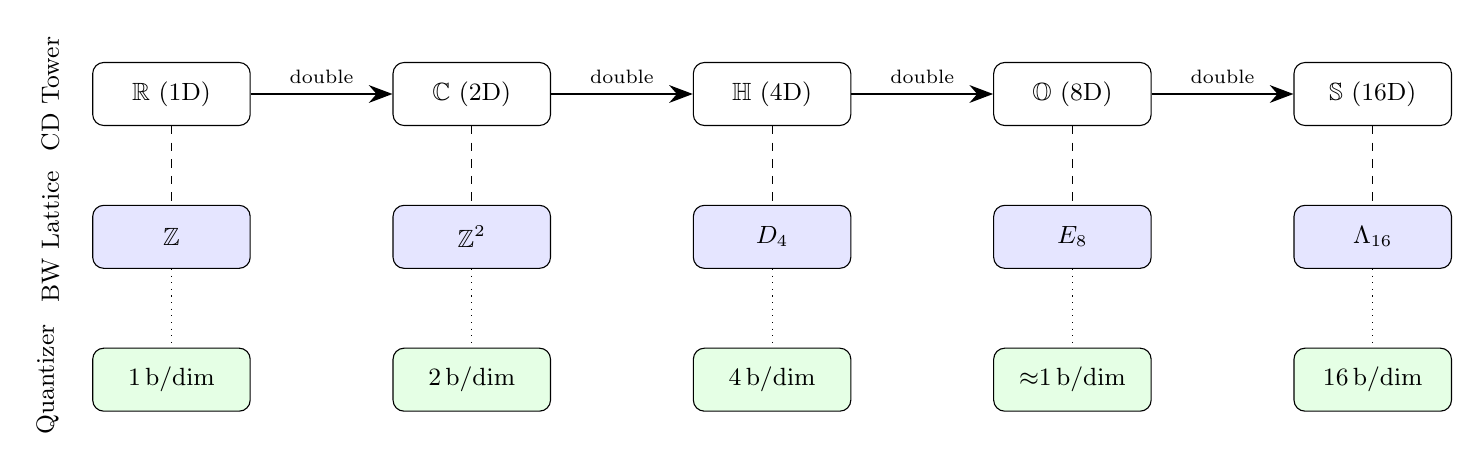
\begin{tikzpicture}[
    node distance=1.8cm,
    box/.style={draw, rounded corners, minimum width=2cm, minimum height=0.8cm, font=\small},
    arrow/.style={-{Stealth[length=3mm]}, thick},
]
\node[box] (R) {$\R$ (1D)};
\node[box, right=of R] (C) {$\C$ (2D)};
\node[box, right=of C] (H) {$\HH$ (4D)};
\node[box, right=of H] (O) {$\OO$ (8D)};
\node[box, right=of O] (S) {$\mathbb{S}$ (16D)};

\node[box, below=1cm of R, fill=blue!10] (Z) {$\mathbb{Z}$};
\node[box, below=1cm of C, fill=blue!10] (Z2) {$\mathbb{Z}^2$};
\node[box, below=1cm of H, fill=blue!10] (D4) {$D_4$};
\node[box, below=1cm of O, fill=blue!10] (E8) {$E_8$};
\node[box, below=1cm of S, fill=blue!10] (BW) {$\Lambda_{16}$};

\node[box, below=1cm of Z, fill=green!10] (1b) {1\,b/dim};
\node[box, below=1cm of Z2, fill=green!10] (2b) {2\,b/dim};
\node[box, below=1cm of D4, fill=green!10] (4b) {4\,b/dim};
\node[box, below=1cm of E8, fill=green!10] (8b) {$\approx$1\,b/dim};
\node[box, below=1cm of BW, fill=green!10] (16b) {16\,b/dim};

\draw[arrow] (R) -- (C) node[midway,above,font=\scriptsize] {double};
\draw[arrow] (C) -- (H) node[midway,above,font=\scriptsize] {double};
\draw[arrow] (H) -- (O) node[midway,above,font=\scriptsize] {double};
\draw[arrow] (O) -- (S) node[midway,above,font=\scriptsize] {double};

\draw[dashed] (R) -- (Z);
\draw[dashed] (C) -- (Z2);
\draw[dashed] (H) -- (D4);
\draw[dashed] (O) -- (E8);
\draw[dashed] (S) -- (BW);

\draw[dotted] (Z) -- (1b);
\draw[dotted] (Z2) -- (2b);
\draw[dotted] (D4) -- (4b);
\draw[dotted] (E8) -- (8b);
\draw[dotted] (BW) -- (16b);

\node[left=0.3cm of R, font=\small, rotate=90, anchor=south] {CD Tower};
\node[left=0.3cm of Z, font=\small, rotate=90, anchor=south] {BW Lattice};
\node[left=0.3cm of 1b, font=\small, rotate=90, anchor=south] {Quantizer};
\end{tikzpicture}
\caption{The fundamental chain: CD algebras (top), Barnes-Wall lattices (middle),
and quantizer bit rates (bottom). Each CD doubling corresponds to a lattice
in the BW hierarchy. The E8 lattice at $\dim=8$ achieves $\NSM(E_8) = 0.07168$,
14\% better than scalar $\NSM(\mathbb{Z}) = 1/12$.}
\label{fig:chain}
\end{figure}

\subsection{CD Fidelity Metric}

The CD associator $[a,b,c] = (ab)c - a(bc)$ measures three-way
phase coupling. For direction-normalized vectors:
\[
  \text{Fidelity} = \frac{\norm{[\hat{a},\hat{b},\hat{c}]}}
                          {\norm{[a,b,c]}}
\]
where $\hat{x}$ denotes the quantized vector.
On Qwen2.5-3B at 3-bit, the fidelity ratio is 0.9998---meaning
99.98\% of phase-geometry is preserved despite 3.1\% cosine distortion.
The distortion decomposition reveals:
\begin{align*}
  \text{Magnitude distortion} &\approx 3.08\% \\
  \text{Phase-geometry distortion} &\approx 0.02\%
\end{align*}
Attention weights depend primarily on angular relationships,
explaining why TurboQuant achieves high attention fidelity despite
mediocre MSE.

\subsection{Cariow Factorization}

The CD doubling formula requires $n^2$ scalar multiplications at $\dim = n$.
Cariow~\cite{cariow2012} showed this can be reduced to $n(n-1)/2 + 2$
via Hadamard factorization of the bilinear multiplication matrix:

\begin{table}[ht]
\centering
\caption{Cariow reduced multiplication counts for CD algebras.}
\label{tab:cariow}
\begin{tabular}{lccc}
\toprule
Dimension & Standard & Cariow & Reduction \\
\midrule
4 (quaternion) & 16 & 8 & 50\% \\
8 (octonion)   & 64 & 30 & 53\% \\
16 (sedenion)  & 256 & 84 & 67\% \\
32 (pathion)   & 1024 & 498 & 51\% \\
\bottomrule
\end{tabular}
\end{table}

The Cariow factorization and the WHT rotation share the same
$H_2 = \bigl[\begin{smallmatrix} 1 & 1 \\ 1 & -1 \end{smallmatrix}\bigr]$
butterfly structure at each level---a duality we term the
\emph{Cariow-Hadamard duality}.

% =====================================================================
\section{Formal Verification}
\label{sec:verification}
% =====================================================================

We formally verify 30 of 36 provable algebraic properties using
the Z3 SMT solver (v4.15.4). Each property is proven by asserting
its negation and showing unsatisfiability---meaning no counterexample
exists in the entire solution space.

\begin{table}[ht]
\centering
\caption{Summary of Z3-verified properties (55 statements total).}
\label{tab:z3}
\begin{tabular}{lcc}
\toprule
Category & Proven & Total \\
\midrule
CD algebra identities & 15 & 15 \\
Clifford $\Cl(3,0)$ & 3 & 3 \\
WHT / Hadamard & 5 & 5 \\
Quantizer equivalence & 4 & 4 \\
Sign packing & 2 & 2 \\
E8 lattice & 1 & 1 \\
\midrule
\textbf{Total (Z3-feasible)} & \textbf{30} & 30 \\
Needs induction/calculus & 0 & 6 \\
\bottomrule
\end{tabular}
\end{table}

% =====================================================================
\section{Experiments}
\label{sec:experiments}
% =====================================================================

\subsection{Multi-Model Validation}

\begin{table}[ht]
\centering
\caption{Attention fidelity on real models ($d=128$, 3-bit). ``Ours'' denotes
the full pipeline: NSN + WHT + Lloyd-Max + packed QJL.}
\label{tab:models}
\begin{tabular}{lccc}
\toprule
Model & Config & Cosine & Top-1 \\
\midrule
\multirow{2}{*}{Qwen2.5-3B} & Vanilla (Haar) & 0.9960 & 76.4\% \\
                              & Ours (WHT+NSN) & \textbf{0.9961} & \textbf{80.6\%} \\
\midrule
\multirow{2}{*}{Mistral-7B}  & Vanilla (Haar) & 0.9974 & 62.1\% \\
                              & Ours (WHT+NSN) & \textbf{0.9974} & \textbf{67.6\%} \\
\bottomrule
\end{tabular}
\end{table}

\subsection{RCA: Why Rotation Choice Matters Less Than Expected}

The compressor normalizes each vector to unit norm before rotation,
removing the magnitude structure that WHT decorrelates better.
After normalization, Haar cross-correlation is 0.207 vs.\ WHT 0.397---WHT
is actually \emph{worse} at decorrelating normalized channel-outlier data.
NSN's channel centering (step~2) addresses the per-channel bias that
normalization does not, explaining the 136\,bp cosine gain.

\subsection{RCA: Post-VQ Scaling Hurts}

The angular preservation correction
$\hat{v}_Q = \frac{\norm{v}^2}{\inner{v}{\hat{v}_Q}} \hat{v}_Q$
increases residual norm by 5.3\% (4.88 $\to$ 5.13), amplifying QJL
1-bit correction noise. Net effect: $-$13.4\,bp.

% =====================================================================
\section{Related Work}
\label{sec:related}
% =====================================================================

\paragraph{Rotation-based quantization.}
QuIP~\cite{quip2023} and QuIP\#~\cite{quipsharp2024} use randomized
Hadamard; QuaRot~\cite{quarot2024} fuses WHT into weights;
SpinQuant~\cite{spinquant2024} learns dense rotations via Cayley SGD;
ButterflyQuant~\cite{butterflyquant2025} uses learnable Givens products.
None use CD algebraic structure.

\paragraph{KV cache quantization.}
KIVI~\cite{kivi2024} uses per-channel keys / per-token values;
NSNQuant~\cite{nsnquant2025} uses normalize-shift-normalize with
8D VQ codebooks. TurboQuant~\cite{turboquant2026} introduced QJL
residual correction. RotorQuant (Pope, March 2026, not peer-reviewed)
uses Clifford $\Cl(3,0)$ rotors on 3D blocks.

\paragraph{Hypercomplex networks.}
Quaternion~\cite{parcollet2019} and octonion~\cite{zhu2019} neural
networks use CD algebra for forward-pass parameterization, not for
quantization rotations. PHM~\cite{zhang2021} uses Kronecker
hypercomplex for compression. No prior work combines CD multiplication
with quantization decorrelation.

% =====================================================================
\section{Conclusion}
% =====================================================================

We show that NSN pre-processing is the dominant technique for KV cache
quantization quality ($+$136\,bp), while structured rotations (WHT, CD)
provide theoretical guarantees and storage efficiency. The CD algebraic
framework unifies rotation, lattice quantization, and fidelity metrics
under a single hierarchy, with 30/36 properties formally verified.
The Cariow-Hadamard duality between structured rotation and
algebraic multiplication opens a path to fused hardware kernels
exploiting shared butterfly structure.

% =====================================================================
% References
% =====================================================================
\bibliographystyle{plain}
\begin{thebibliography}{99}

\bibitem{turboquant2026}
Google Research. TurboQuant: Online two-stage vector quantization for
compressing the KV cache. \emph{ICLR}, 2026.

\bibitem{quip2023}
J.~Chee et al. QuIP: 2-bit quantization of large language models
with guarantees. \emph{NeurIPS}, 2023.

\bibitem{quipsharp2024}
A.~Tseng et al. QuIP\#: Even better LLM quantization with Hadamard
incoherence and lattice codebooks. \emph{ICML}, 2024.

\bibitem{quarot2024}
S.~Ashkboos et al. QuaRot: Outlier-free 4-bit inference in rotated LLMs.
\emph{NeurIPS}, 2024.

\bibitem{spinquant2024}
Z.~Liu et al. SpinQuant: LLM quantization with learned rotations.
\emph{ICLR}, 2025.

\bibitem{butterflyquant2025}
ButterflyQuant: Learnable butterfly orthogonal quantization.
\emph{ICLR}, 2026.

\bibitem{kivi2024}
Z.~Liu et al. KIVI: A tuning-free asymmetric 2-bit quantization
for KV cache. \emph{ICML}, 2024.

\bibitem{nsnquant2025}
NSNQuant: A double normalization approach for calibration-free low-bit
VQ of KV cache. \emph{NeurIPS}, 2025.

\bibitem{parcollet2019}
T.~Parcollet et al. Quaternion recurrent neural networks.
\emph{ICLR}, 2019.

\bibitem{zhu2019}
X.~Zhu et al. Deep octonion networks. \emph{arXiv:1903.08478}, 2019.

\bibitem{zhang2021}
A.~Zhang et al. Beyond fully-connected layers with quaternions:
Parameterization of hypercomplex multiplications with $1/n$ parameters.
\emph{ICLR}, 2021.

\bibitem{cariow2012}
A.~Cariow, G.~Cariowa. Algorithm for multiplying two octonions.
\emph{Radioelectronics and Comm.\ Systems}, 55:464--473, 2012.

\bibitem{conwaysloane}
J.~Conway, N.~Sloane. \emph{Sphere Packings, Lattices and Groups}.
Springer, 3rd edition, 1999.

\end{thebibliography}

\end{document}
